% This file was created with tikzplotlib v0.10.1.
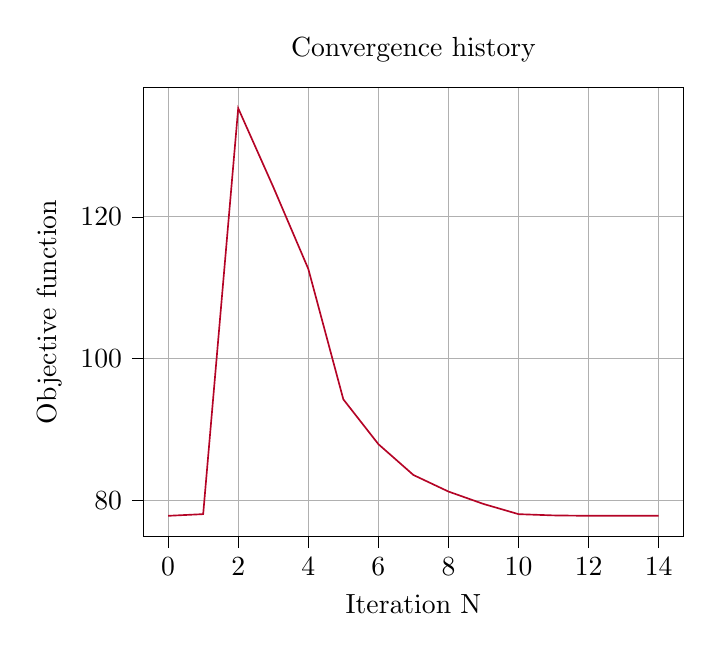
\begin{tikzpicture}

\definecolor{darkgray176}{RGB}{176,176,176}
\definecolor{firebrick180438}{RGB}{180,4,38}

\begin{axis}[
tick align=outside,
tick pos=left,
title={Convergence history},
x grid style={darkgray176},
xlabel={Iteration N},
xmajorgrids,
xmin=-0.7, xmax=14.7,
xtick style={color=black},
y grid style={darkgray176},
ylabel={Objective function},
ymajorgrids,
ymin=74.9041925437389, ymax=138.212906882091,
ytick style={color=black}
]
\addplot [semithick, firebrick180438]
table {%
0 77.7818617380553
1 78.0214491937485
2 135.33523804853
3 124.226200218441
4 112.655775229008
5 94.2308299000817
6 87.9026459908608
7 83.5458236829191
8 81.2093575451013
9 79.4570364643508
10 78.0172021020735
11 77.8403320273127
12 77.7828104296361
13 77.781870231547
14 77.7818613773004
};
\end{axis}

\end{tikzpicture}
